\externaldocument{../3/chapter_modeling}
\externaldocument{../4/chapter_algorithm}
\startchapter{Feature Prototype On Atlantis}
\label{chapter:newsol}
In this section, I describe the design of the feature prototype of communication identification from the dual\_trace. This feature is implemented on Atlantis and is built on top of Atlantis' other features, such as ``memory reconstruction", ``function inspect" and ``views synchronization". Atlantis is an assembly trace analysis environment. It provides many powerful and novel features to assist assembly level execution trace analysis.\cite{huang2017atlantis} This prototype implemented some of the algorithms described in Chapter\ref{chapter:alo} as well as the user interfaces.

This prototype consists of four main components: 1) user defined setting for defining the concerned communication methods' description. 2) a view that can parallelly present both traces in the dual\_trace. 3) two identification features: Event Stream identification and communication identification. 4) identification result navigation.


\section{User Defined Communication Method Description}\label{functionset}
In Chapter\ref{chapter:alo}, I defined the communication method description which is a set of function descriptions of a specific communication method. The communication method descriptions restrict how the communication looks like in the dual\_trace and how they can be identified.

However, the communication method description for a communication method can be different depends on the implementation solution of the method. Furthermore, there are so many communication methods in the real world, there is no way that we can define all of them for the users. Instead, a configuration file in Json format is used for the users to define their concerned communication methods and the corresponding description. This setting file will be the input for the communication identification. All concerned communication methods can be listed in this file. The identification features implemented in this prototype iterate all methods in the Json configuration file named ``communicationMethods.json" and identify the selected ones. This configuration includes the communication method and their function descriptions. A default template is given for user reference, this default template is generated by Atlantis when it was launched and stored in the .tmp folder in the trace analysis project folder. The users can modify this template as to the communication method of interest. The default template example can be find in Section\ref{funcset}.

\subsection{Communication Methods' Implementation in Windows}\label{windows}
In this section, I present the result of investigation about the implementation of the four communication methods: Named Pipe, Message Queue, TCP and UDP in Windows. By this investigation, the communication descriptions of these methods can be designed.

In the investigation, I reviewed the Windows APIs of the communication methods and their example code. 

Windows API set is very sophisticated and multiple solutions are provided to fulfil a communication method. It is impossible to enumerate all solutions for each communication method. I only investigated the most basic usage provided in Windows documentation. For each communication method, a system function list is provided for reference as the communication method description. The functions in the description are supported in most Windows operating systems, such as Windows 8, Window 7. The provided function descriptions for a communication method should not be considered as the only combination or solution for that communication method. With the understanding of this, it should be fairly easy to draw out lists for other solutions or other communication methods. 

Moreover, the instances of the descriptions only demonstrate Windows C++ APIs. But the idea of the description is generalizable to other operating systems with the effort of understanding the APIs of those operating systems.

\subsubsection{Windows Calling Convention}
The Windows calling convention is important to know in this research. The communication identification relies not only on the system function names but also the key parameter values. In the assembly level execution traces, the parameter values is captured in the memory changes and register changes of the instructions. The calling convention helps us to understand where the parameters are stored so that we can find them in the memory state of while emulate the execution of the trace. Calling Convention is different for operating systems and the programming language. The Microsoft* x64 example calling convention is listed in Appendix \ref{convention} since we used dual-trace from Microsoft* x64 for case study in this work.

\subsubsection{Named Pipes}
In Windows, a named pipe is a communication method for the pipe server and one or more pipe clients. The pipe has a name, can be one-way or duplex. Both the server and clients can read or write into the pipe.\cite{WinNamedpipe} In this work, I only consider one server versus one client communication. One server to multiple clients scenario can always be divided into multiple server and client communications thanks to the characteristic that each client and server communication has a separate conduit. The server and client are endpoints in the communication. We call the server ``server endpoint" while the client ``client endpoint".  The server endpoint and client endpoint of a named pipe share the same pipe name, but each endpoint has its own buffers and handles. 

There are two modes for data transfer in the named pipe communication method, synchronous and asynchronous.  Modes affect the functions used to complete the send and receive operation. I list the related functions for both synchronous mode and asynchronous mode. The create channel functions for both modes are the same but with different input parameter value. The functions for send and receive message are also the same for both cases. However, the operation of the send and receive functions are different for different modes. In addition, an extra function \textit{GetOverlappedResult} is being called to check if the sending or receiving operation finish, the output message will be stored in the overlap structure whose memory address saved in the function's output parameter Overlap Structure Address. Table\ref{synfunctions} lists the functions of the events for synchronous mode while Table\ref{asynfunctions} lists the functions of the events for the asynchronous mode for a Named pipe communication.

\begin{table}[H]
  \centering
  \caption{Function Descriptions for Synchronous Named Pipe}
  \label{synfunctions}
  \begin{tabular}{|l|l|l|l|l|l|}
      \hline
       \multirow{2}{*}{{\textbf{Name}}} & \multirow{2}{*}{{\textbf{Type}}} & \multicolumn{4}{c|}{\textbf{Parameter Description}}  \\
        \cline{3-6} 
       & & \textbf{Parameter}& \textbf{Register}& \textbf{In or Out} &  \textbf{Buffer Or Value}  \\
       \hline
       \multirow{2}{*}{CreateNamedPipe}
       &\multirow{2}{*}{open} &  Handle & RAX: & Out & Value\\
        \cline{3-6} 
       & & FileName & RCX & In & Address\\
      \hline         
      \multirow{2}{*}{CreateFile}
       &\multirow{2}{*}{open} &  Handle & RAX: & Out & Value\\
        \cline{3-6} 
       & & FileName & RCX & In & Address\\
      \hline              
      \multirow{3}{*}{WriteFile}
       &\multirow{3}{*}{send} &  Handle & RCX & In & Value\\
        \cline{3-6} 
       & & SendBuffer & RDX & In & Address\\
        \cline{3-6} 
       & & MessageLength & R9 & Out & Value\\
      \hline            
      \multirow{3}{*}{ReadFile}
       &\multirow{3}{*}{receive} &  Handle & RCX & In & Value\\
        \cline{3-6} 
       & & RecvBuffer & RDX & In & Address\\
        \cline{3-6} 
       & & MessageLength & R9 & Out & Value\\
      \hline            
      CloseHandle &
       close &  Handle & RCX & In & Value\\
      \hline            
      DisconnectNamedPipe &
      close &  Handle & RCX & In & Value\\
      \hline               
  \end{tabular}
\end{table}

\begin{table}[H]
  \centering
  \caption{Function Descriptions for Asynchronous Named Pipe}
  \label{asynfunctions}
  \begin{tabular}{|l|l|l|l|l|l|}
      \hline
       \multirow{2}{*}{{\textbf{Name}}} & \multirow{2}{*}{{\textbf{Type}}} & \multicolumn{4}{c|}{\textbf{Parameter Description}}  \\
        \cline{3-6} 
       & & \textbf{Parameter}& \textbf{Register}& \textbf{In or Out} &  \textbf{Buffer Or Value}  \\
       \hline
       \multirow{2}{*}{CreateNamedPipe}
       &\multirow{2}{*}{open} &  Handle & RAX: & Out & Value\\
        \cline{3-6} 
       & & FileName & RCX & In & Address\\
      \hline         
      \multirow{2}{*}{CreateFile}
       &\multirow{2}{*}{open} &  Handle & RAX: & Out & Value\\
        \cline{3-6} 
       & & FileName & RCX & In & Address\\
      \hline              
      \multirow{3}{*}{WriteFile}
       &\multirow{3}{*}{send} &  Handle & RCX & In & Value\\
        \cline{3-6} 
       & & SendBuffer & RDX & In & Address\\
        \cline{3-6} 
       & & MessageLength & R9 & Out & Value\\
      \hline            
      \multirow{3}{*}{ReadFile}
       &\multirow{3}{*}{receive} &  Handle & RCX & In & Value\\
        \cline{3-6} 
       & & RecvBuffer & RDX & In & Address\\
        \cline{3-6} 
       & & MessageLength & R9 & Out & Value\\
      \hline  
      \multirow{2}{*}{GetOverlappedResult}
       &\multirow{2}{*}{send/receive} &  Handle & RCX: & In & Value\\
        \cline{3-6} 
       & & OverlapStruct & RDX & Out & Address\\
      \hline            
      CloseHandle &
       close &  Handle & RCX & In & Value\\
      \hline            
      DisconnectNamedPipe &
      close &  Handle & RCX & In & Value\\
      \hline               
  \end{tabular}
\end{table}

\subsubsection{Message Queue}
Similar to Named Pipe, Message Queue's implementation in Windows also has two modes, synchronous and asynchronous. Moreover, the asynchronous mode further divides into two operations, one with callback function while the other without. With the callback function, the callback function would be called when the send or receive operations finish. Without callback function, the general function \textit{MQGetOverlappedResult} should be called by the endpoints to check if the message sending or receiving operation finish, the output message will be stored in the overlap structure whose memory address saved in the function's output parameter Overlap Structure Address. Table\ref{msmqsynfunctions} lists the function descriptions for synchronous mode while Table\ref{msmqasynfunctions} list the function descriptions for the asynchronous mode without callback. With callback function situation is not elaborated here.

\begin{table}[H]
  \centering
  \caption{Function Descriptions for Synchronous Message Queue}
  \label{msmqsynfunctions}
  \begin{tabular}{|l|l|l|l|l|l|}
      \hline
       \multirow{2}{*}{{\textbf{Name}}} & \multirow{2}{*}{{\textbf{Type}}} & \multicolumn{4}{c|}{\textbf{Parameter Description}}  \\
        \cline{3-6} 
       & & \textbf{Parameter}& \textbf{Register}& \textbf{In or Out} &  \textbf{Buffer Or Value}  \\
       \hline
       \multirow{2}{*}{MQOpenQueue}
       &\multirow{2}{*}{open} &  Handle & RAX: & Out & Value\\
        \cline{3-6} 
       & & QueueName & RCX & In & Address\\
      \hline         
      \multirow{2}{*}{CreateFile}
       &\multirow{2}{*}{open} &  Handle & RAX: & Out & Value\\
        \cline{3-6} 
       & & FileName & RCX & In & Address\\
      \hline              
      \multirow{2}{*}{MQSendMessage}
       &\multirow{2}{*}{send} &  Handle & RCX & In & Value\\
        \cline{3-6} 
       & & MessageStruct & RDX & In & Address\\
      \hline            
      \multirow{2}{*}{MQReceiveMessage}
       &\multirow{2}{*}{receive} &  Handle & RCX & In & Value\\
        \cline{3-6} 
       & & MessageStruct & R9 & In & Address\\
      \hline   
     MQCloseQueue &
       close &  Handle & RCX & In & Value\\
      \hline               
  \end{tabular}
\end{table}

\begin{table}[H]
  \centering
  \caption{Function Descriptions for Asynchronous Message Queue}
  \label{msmqasynfunctions}
  \begin{tabular}{|l|l|l|l|l|l|}
    \hline
     \multirow{2}{*}{{\textbf{Name}}} & \multirow{2}{*}{{\textbf{Type}}} & \multicolumn{4}{c|}{\textbf{Parameter Description}}  \\
      \cline{3-6} 
     & & \textbf{Parameter}& \textbf{Register}& \textbf{In or Out} &  \textbf{Buffer Or Value}  \\
     \hline
     \multirow{2}{*}{MQOpenQueue}
     &\multirow{2}{*}{open} &  Handle & RAX: & Out & Value\\
      \cline{3-6} 
     & & QueueName & RCX & In & Address\\
    \hline         
    \multirow{2}{*}{CreateFile}
     &\multirow{2}{*}{open} &  Handle & RAX: & Out & Value\\
      \cline{3-6} 
     & & FileName & RCX & In & Address\\
    \hline              
    \multirow{2}{*}{MQSendMessage}
     &\multirow{2}{*}{send} &  Handle & RCX & In & Value\\
      \cline{3-6} 
     & & MessageStruct & RDX & In & Address\\
    \hline            
    \multirow{2}{*}{MQReceiveMessage}
     &\multirow{2}{*}{receive} &  Handle & RCX & In & Value\\
      \cline{3-6} 
     & & MessageStruct & R9 & In & Address\\
    \hline            
    MQGetOverlappedResult &
     receive/send &  OverlapStrAndHandle & RCX & In/Out & Address\\
     \hline            
     MQCloseQueue &
      close &  Handle & RCX & In & Value\\
    \hline               
\end{tabular}
\end{table}


    
\subsubsection{TCP and UDP}
In Windows programming, these two methods shared the same set of APIs regardless the input parameter values and operation behaviour are different. In Windows socket solution, one of the two endpoints is the server while the other one is the client. Table \ref{tcpupdfunctions} lists the functions of a UDP or TCP communication. 

\begin{table}[H]
  \centering
  \caption{Function Descriptions for for TCP and UDP}
  \label{tcpupdfunctions}
  \begin{tabular}{|l|l|l|l|l|l|}
    \hline
     \multirow{2}{*}{{\textbf{Name}}} & \multirow{2}{*}{{\textbf{Type}}} & \multicolumn{4}{c|}{\textbf{Parameter Description}}  \\
      \cline{3-6} 
     & & \textbf{Parameter}& \textbf{Register}& \textbf{In or Out} &  \textbf{Buffer Or Value}  \\
     \hline
     socket & open &  Handle & RAX: & Out & Value\\
    \hline   
    \multirow{2}{*}{bind}
    &\multirow{2}{*}{open} &  Handle & RCX: & In & Value\\
     \cline{3-6} 
    & & ServerAddAndPort & RDX & Out & Address\\
   \hline 
   \multirow{3}{*}{accept}
   &\multirow{3}{*}{open} &  ChildHandle & RAX & Out & Vaule\\
    \cline{3-6} 
   & & Handle & RCX & In & Value\\
   \cline{3-6} 
   & & ClientAddAndPort & RDX & In & Value\\
  \hline 
  \multirow{2}{*}{send}
  &\multirow{2}{*}{send} &  Handle & RCX: & In & Value\\
   \cline{3-6} 
  & & SendBuffer & RCX & In & Address\\
 \hline       
    \multirow{2}{*}{recv}
     &\multirow{2}{*}{receive} &  Handle & RAX & In & Value\\
      \cline{3-6} 
     & & RecvBuffer & RCX & Out & Address\\
    \hline                        
     closesocket &
      close &  Handle & RCX & In & Value\\
    \hline               
\end{tabular}
\end{table}

\section{Parallel Editor View For Dual\_Trace}
The dual\_trace consist of two execution traces which are interacting with each other. Presenting them in the same view makes the analysis for the user much easier. To open parallel editor view, the user need to open one trace as the normal one and the other as the dual\_trace of the opened one. A new menu option in the project navigation view are added to open the second trace as the dual\_trace of the active trace. The implementation of the parallel editor take the advantage of the existing SWT of Eclipse plug-in development. The detail of the implementation can be found in Appendix \ref{paralleleditor}. Figure \ref{opendualtracemenu} shows this menu option and Figure \ref{paralleleditor} shows the parallel editor view.

\begin{figure}[H]
\centerline{\includegraphics[scale=0.55]{Figures/opendualtracemenu}}
 \caption{Menu Item for opening Dual\_trace}
\label{opendualtracemenu}
\end{figure}

\begin{figure}[H]
\centerline{\includegraphics[scale=0.6]{Figures/paralleleditor}}
 \caption{Parallel Editor View}
\label{paralleleditor}
\end{figure}



\section{Identification Features}
I implemented two identification features, one is stream identification for both traces in the dual\_trace, the other is the communication identification. These two features implemented the ``event stream extraction algorithm" and ``event stream matching algorithm" designed in Chapter\ref{chapter:alo}. The implementation of these two identification features relies on the existing ``function inspect" feature of Atlantis. The called functions' name can be inspected  by  search of the symbolic name in the executable binary or any DLLs which used by the program at the time when it is traced. By importing the DLLs and executable binary, Atlantis can recognize the function call from the execution trace by the function names. Therefore the corresponding Dlls or executable binaries for both traces in the dual\_trace have to be loaded into Atlantis before conducting the identification.

A new menu ``Dual\_trace Tool" with three menu options is designed for these two identification features. In this menu, two options are for conducting the identification which are ``Stream Identification" and ``Communication Identification" while one is for loading the DLLs and executable binary which is ``Load Library Exports". Currently, the ``Load library export" function can only load libraries for the trace in the active editor. So this item in the menu has to be run twice separately for each trace of the dual\_trace.  Figure\ref{dualtracetoolmenu} shows this new menu in Atlantis. When the user perform any of the identification features, there is the prompt dialog as shown in Figure \ref{methods} which asks the user what communication methods they want to identify from the dual\_trace. This list is provided by the configuration file I mention in Section \ref{functionset}. The user can select one or multiple methods. 

\begin{figure}[H]
\centerline{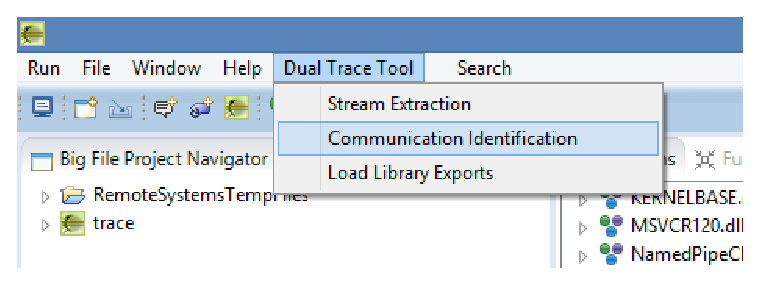
\includegraphics{Figures/dualtracetoolmenu}}
 \caption{Dual\_trace Tool Menu}
\label{dualtracetoolmenu}
\end{figure}

\begin{figure}[H]
\centerline{\includegraphics[scale=0.8]{Figures/methods}}
 \caption{Prompt Dialog for Communication Selection}
\label{methods}
\end{figure}

A new view named ``Communication" is designed for presenting the result of the identification of streams and communications. Since the user can have multiple selection for communication methods they concern, the output identification result contains all the identified communications or streams of all the concerned communication methods and the identified results are clustered by methods. There are two sub tables in this view, the left one is for the stream identification result while the left one is for communication identification result. The reason for putting this two result in the same view is for easy access and comparison of the data for the users. Figure \ref{idenview} shows this view with result data in it. Each time when the user rerun the identification features the result in the corresponding table will be refreshed to show only the latest identification result. But the other table will not be affected. For example, if the user run the ``Stream Identification" feature first, the stream identification result will show on the left table of the view. And then the user run the ``communication Identification", the communication identification result will be shown on the right table while the left one still holding the last stream identification result.

\begin{figure}[H]
\centerline{\includegraphics[scale=0.7]{Figures/idenview}}
 \caption{Communication View for Showing Identification Result}
\label{idenview}
\end{figure}

\section{Identification Result View and Result Navigation}
Atlantis is a analysis environment that has various views to allow user access to different information from the trace, such as the memory and register state of the current instruction line. Moreover, these views synchronize automatically with the editor view. These functionality and information also benefit the communication analysis of the dual\_trace. Providing the user a way to navigate from the identified result to the traces in the editors allows them to take advantage of the current existing functionality of Atlantis and make their analysis of the dual\_trace more efficient.

In the result list, each event entry is corresponding to a function call. The functions were called at function call line and all the inputs of the function calls can be recovered from the memory state of this instruction line. The functions returned at the return instruction lines, all the outputs of the function calls can be recovered in the memory state of the the return instruction line. From the event entries, this implementation provide two different ways for the user to navigate back to where the function begins and ends. When the user ``double click" on an entry, it will bring the user to the start line of the function in the corresponding trace editor. When the the right click on the event entry, a prompted menu with the option ``Go To Line of Function End" will show up as in Figure \ref{gotoend}. Clicking on this option will bring the user to the return line of this function in the trace editor. All other views update immediately with this navigation. 

\begin{figure}[H]
\centerline{\includegraphics{Figures/gotoend}}
 \caption{Right Click Menu on Event Entry}
\label{gotoend}
\end{figure}

Moreover, the ``remove" option as shown in Figure \ref{remove} in the right click menu on the ``stream“ or ``communication" entries is provided for the user to remove the selected ``stream" or ``communication" entry. This provides the user the flexibility to get rid of the data that they don't care.

\begin{figure}[H]
\centerline{\includegraphics[scale=0.7]{Figures/remove}}
 \caption{Right Click Menu on Event Entry}
\label{remove}
\end{figure}

